\chapter{ROS AND MOVEIT!}
\label{ch:ROS AND MOVEIT!}
In this chapter, we make a brief introduction to ROS \cite{o2014gentle}, system we used to program the robot arm, the force/torque sensor and the gripper. We also talk about MoveIt!, which provides the functionality for manipulation in ROS.

\section{Introduction to ROS}
The rapid progress on the development of robotic systems has caused that robots still present some significant challenges for software developers. ROS, Robot Operating System, is a platform that is intended to ease some of these difficulties. The official description of ROS is:
\begin{quote}
\textit{ROS is an open-source, meta-operating system for your robot. It provides the services you would expect from an operating system, including hardware abstraction, low-level device control, implementation of commonly-used functionality, message-passing between processes, and package management. It also provides tools and libraries for obtaining, building, writing, and running code across multiple computers. \cite{o2014gentle}}
\end{quote}

Creating truly robust, general-purpose robot software is hard. From the robot's perspective, problems that seem trivial to humans often vary wildly between instances of tasks and environments. Dealing with these variations is so hard that no single individual, laboratory, or institution can hope to do it on their own \cite{ros}.

The Robot Operating System (ROS) is a flexible framework for writing robot software. It is a collection of tools, libraries, and conventions that aim to simplify the task of creating complex and robust robot behavior across a wide variety of robotic platforms \cite{cashmore2015rosplan}.

The goal of ROS is not to be a framework with the most features. Instead, the primary goal of ROS is to support code reuse in robotics research and development. ROS is a distributed framework of processes (aka Nodes) that enables executables to be individually designed and loosely coupled at runtime. These processes can be grouped into Packages and Stacks, which can be easily shared and distributed. ROS also supports a federated system of code Repositories that enable collaboration to be distributed as well. This design, from the filesystem level to the community level, enables independent decisions about development and implementation, but all can be brought together with ROS infrastructure tools \cite{wikiros}.

As a result, ROS was built from the ground up to encourage collaborative robotics software development. For example, one laboratory might have experts in mapping indoor environments, and could contribute a world-class system for producing maps. Another group might have experts at using maps to navigate, and yet another group might have discovered a computer vision approach that works well for recognizing small objects in clutter. ROS was designed specifically for groups like these to collaborate and build upon each other's work \cite{ros}.

We can thus say that the advent of new open-source frameworks like ROS has made robotics more accessible to new users, both in research and consumer applications. ROS has revolutionized the developers community, providing it with a set of tools, infrastructure and best practices to build new applications and robots. A key pillar of the ROS effort is the notion of \textit{not re-inventing the wheel} by providing easy to use libraries for different capabilities like navigation, manipulation, control (and more) \cite{koubaa2016robot}.

Figure~\ref{fig:ros} below summarizes ROS:

\begin{figure}[htbp]
	\centering
	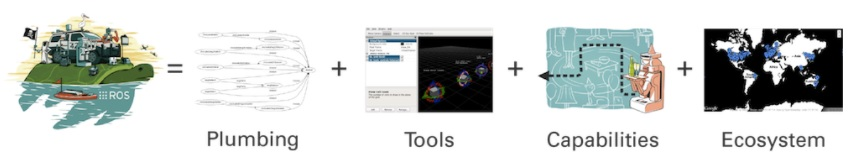
\includegraphics{chapters/figures/ROS/ROS.jpg}
	\caption{ROS Summary.}
	\label{fig:ros}
\end{figure}

\textit{Plumbing:} ROS provides publish-subscribe messaging infrastructure designed to support the quick and easy construction of distributed computing systems.

\textit{Tools:} ROS provides an extensive set of tools for configuring, starting, introspecting, debugging, visualizing, logging, testing, and stopping distributed computing systems.

\textit{Capabilities:} ROS provides a broad collection of libraries that implement useful robot functionality, with a focus on mobility, manipulation, and perception.

\textit{Ecosystem:} ROS is supported and improved by a large community, with a strong focus on integration and documentation. ros.org is a one-stop-shop for finding and learning about the thousands of ROS packages that are available from developers around the world.

 ROS has already been implemented in Python, C++, and Lisp, and there are experimental libraries in Java and Lua \cite{wikiros}.

ROS currently only runs on Unix-based platforms. Software for ROS is primarily tested on Ubuntu and Mac OS X systems, though the ROS community has been contributing support for Fedora, Gentoo, Arch Linux and other Linux platforms. While a port to Microsoft Windows for ROS is possible, it has not yet been fully explored \cite{wikiros}.

As this project focuses on robotic manipulation, let's now talk about MoveIt! which provides the core functionality for manipulation in ROS.

\section{MoveIt!}
MoveIt! is a software for mobile manipulation, incorporating the latest advances in motion planning, manipulation, 3D perception, kinematics, control and navigation. It provides an easy-to-use platform for developing advanced robotic applications, evaluating new robot designs and building integrated robotics products for industrial, commercial, R\&D and other domains \cite{moveit}. 

This software builds on multiple pillars:
\begin{itemize}
\item A library of capabilities: MoveIt! provides a library of robotic capabilities for manipulation, motion planning, control and mobile manipulation.
\item A strong community: A strong community of users and developers that help in maintaining and extending MoveIt! to new applications.
\item Tools: A set of tools that allow new users to integrate MoveIt! with their robots and advanced users to deploy new applications.
\end{itemize}

MoveIt! is the most widely used open-source software for manipulation and has been used on over 65 different robots \cite{koubaa2016robot}. 

\begin{figure}[htbp]
	\centering
	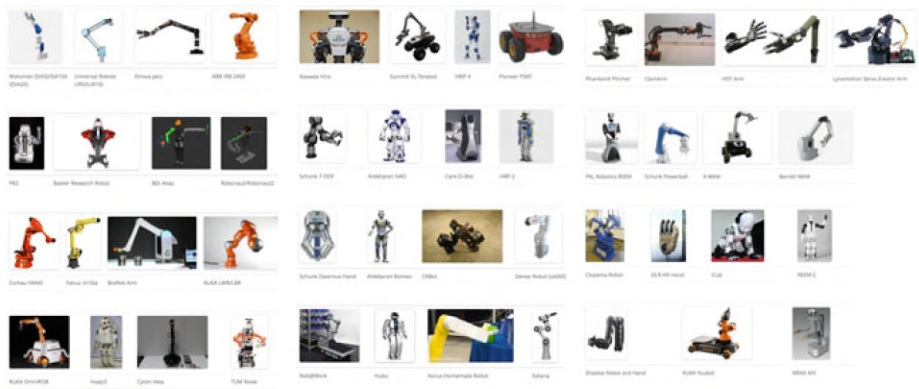
\includegraphics{chapters/figures/ROS/robots_moveit.jpg}
	\caption{Robots using MoveIt!}
	\label{fig:robots_moveit}
\end{figure}

Figure~\ref{fig:robots_moveit} shows a list of robots that MoveIt! has been used with. The robots range from industrial robots from all the leading vendors to research robots from all over the world. The robots include single arm, dual-armed robots, mobile manipulation systems, and humanoide robots. Among these robots, we find the UR10 robot arm which we will be working with. MoveIt! has been used in applications ranging from unstructured autonomous pick and place (with industrial robots like the UR5), mobile manipulation (with the PR2 and other robots), process tasks like painting and welding, with the (simulated) Robonaut robot for target applications in the space station. MoveIt! has been used used by teams in the DARPA Robotics Challenge, the ROS-Industrial Consortium, the Amazon Picking Challenge, the NASA sample retrieval challenge \cite{koubaa2016robot}.

\section{How to control to UR10, Robotiq 3 finger gripper and Robotiq FT300 force/torque sensor through ROS}
In this section, we explain how to control UR10, Robotiq 3 finger gripper and FT300 force/torque sensor through ROS.
%
%For this project, we are working on Ubuntu 16.04.3 LTS with ROS kinetic.

To control UR10 through ROS, we must install the Universal Robots package \cite{urpackage}. Through this package we can establish communication with UR10 controllers. Then, for the communication with Robotiq FT300 force/torque sensor and the 3 finger gripper, we must install Robotiq package \cite{robotiq}. Once we have installed those packages, we can run the executables to establish the connection with the three elements.

To make the connection with UR10 robot, the files shown below must be launched in three different terminals:
\begin{quote}
\textit{roslaunch ur\_modern\_driver ur10\_bringup.launch limited:=true robot\_ip:=192.168.1.102 [reverse\_port:=REVERSE\_PORT]}

\textit{roslaunch ur10\_moveit\_config ur10\_moveit\_planning\_execution.launch limited:=true}

\textit{roslaunch ur10\_moveit\_config moveit\_rviz.launch config:=true}
\end{quote}

Now we can create an executable to move the robot arm through ROS.

The communication with the FT300 is made by typing in two different terminals:
\begin{quote}
\textit{sudo chmod 777 /dev/ttyUSB1}

\textit{rosrun robotiq\_force\_torque\_sensor rq\_sensor}
\end{quote}

And the connection with the gripper is made by typing in other two different terminals:
\begin{quote}
\textit{rosrun robotiq\_s\_model\_control SModelTcpNode.py 192.168.1.11}

\textit{rosrun robotiq\_s\_model\_control SModelSimpleController.py}
\end{quote}

Now, we know how to control the three elements through ROS, so let's figure out which path the end-effector must follow to untie the string.
